\chapter{Introduction to the RV12} \label{introduction-to-the-rv12}

The RISC-V specification provides for multi-threading and multi-core implementations. 
A core is defined as an implementation with its own instruction fetch unit. 
A hardware thread, or \emph{hart}, is defined as a processing engine with its own state. 
A core may contain multiple hardware threads. 
See \href{http://www.riscv.org}{www.riscv.org} for the specifications\footnote{Full reference details of the specifications are documented in section 11}.

The RV12 implements a single core 32/64bit Reduced Instruction Set Computing (RISC) Central Processing Unit (CPU) with a single hardware thread, based on the RISC-V User Instruction Set Architecture v2.2 and Supervisor Instruction Set Architecture v1.9.1 specifications. 
The core is highly configurable, providing the user with a trade-off between area, power, and performance, thus allowing it to be optimized for the intended task.

	See Configurations section for a description of the configuration options and parameters.

\section{Privilege Levels}\label{privilege-levels}

At any time, a hardware thread (\emph{hart}) is running at some privilege level. 
The current privilege level is encoded in one or more Control and Status Registers (CSRs). 
The RISC-V specification defines four privilege levels, where each level provides its own protection and isolation..

\begin{longtable}[]{@{}cclc@{}}
\toprule
	Level & Encoding    & Name             & Abbreviation\tabularnewline
\midrule
\endhead
	0     & \texttt{00} & User/Application & U\tabularnewline
	1     & \texttt{01} & Supervisor       & S\tabularnewline
	2     & \texttt{10} & Hypervisor       & H\tabularnewline
	3     & \texttt{11} & Machine          & M\tabularnewline
\bottomrule
\caption{RISC-V Privilege Levels}
\label{tab:riscv-priv-levels}
\end{longtable}

The highest privilege level is the Machine level. 
This is an inherent trusted level and has access to, and can alter, the whole machine. 
The lowest level is the User/Application level and is considered the least trusted level. 
It is used to protect the rest of the system from malicious applications.

Supervisor mode is used to provide isolation between an operating system and the machine and user levels. 
Hypervisor mode is used to virtualize operating systems.

The RV12 always implements Machine mode and optionally implements User mode and parts of the Supervisor Mode.

\section{Execution Pipeline}\label{execution-pipeline}

The RV12 implements an optimizing 4-stage folded pipeline. 
The classic RISC pipeline consists of 5 stages; instruction fetch (IF), instruction decode (ID), execute (EX), memory access (MEM), and register write-back (WB).

\begin{figure}[hbt]
  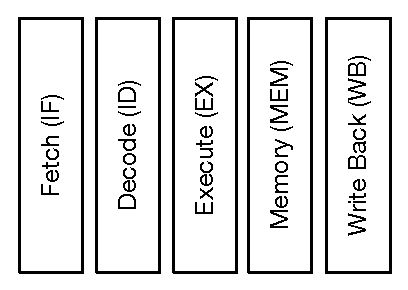
\includegraphics{assets/img/Pipeline-Reg}
  \caption{Classic RISC Pipeline}
\end{figure}

The RV12 implements a modified form of the classic RISC pipeline where the Fetch stage takes 2 cycles to allow time to recode 16bit-compressed instructions and predict branches and jumps. 
The Memory stage is folded into the Execute and Write-Back stages. 
The Decode stage optimizes the instruction stream to allow CPU stalls, instruction execution, and memory accesses to overlap, thereby effectively hiding CPU stalls and improving the CPU's cycles per instruction CPI.

\begin{figure}[hbt]
  
\includegraphics{assets/img/Pipeline-RV12}
  \caption{Modified RV12 Pipeline}
\end{figure}

The RV12 pipeline is capable of executing one instruction per clock cycle by overlapping the execution stages. 
The figure below shows how 5 instructions are being operated on at the same time; this is referred to as `being in flight'. 
Instruction A is the oldest instruction and it's in the Write Back (WB) stage, whereas Instruction E is the
newest instruction and it's in the Instruction Fetch (IF) stage.

\begin{figure}[hbt]
  
\includegraphics{assets/img/Pipeline-Overlap}
  \caption{Overlapping Execution Stages}
\end{figure}

\subsection{Instruction Fetch/Pre-Decode(IF/PD)} \label{instruction-fetchpre-decode-ifpd}

During the instruction fetch stage one instruction is read from the instruction memory, a 16bit-compressed instruction is decoded, and the program counter is updated to point to the next instruction.

\subsection{Instruction Decode (ID)} \label{instruction-decode-id}

During the instruction decode stage the Register File is accessed and the bypass controls are determined.

\subsection{Execute (EX)} \label{execute-ex}

During the Execute stage the result is calculated for an ALU, MUL, DIV instruction, the memory accessed for a Load/Store instruction, and branches and jumps are calculated and checked against their predicted outcomes.

\subsection{Write Back (WB)} \label{write-back-wb}

During the Write Back stage the result from the Execution stage is written into the Register File.

\section{Branch Prediction Unit} \label{branch-prediction-unit}

The RV12 can execute one instruction every clock cycle. 
However due to the pipeline architecture each instruction takes several clock cycles to complete. 
When a branch instruction is decoded its conditions and outcome are not known and waiting for the branch outcome before continuing fetching new instructions would cause excessive processor stalls, affecting the processor's performance.

Instead of waiting the processor predicts the branch's outcome and continues fetching instructions from the predicted address.
When a branch is predicted wrong, the processor must flush its pipeline and restart fetching from the calculated branch address. 
The processor's state is not affected because the pipeline is flushed and therefore none of the incorrectly fetched instructions is actually executed. 
However the branch prediction may have forced the Instruction Cache to load new instructions. 
The Instruction Cache state is NOT restored, meaning the predicted instructions remain in the Instruction Cache.

The RV12 has an optional Branch Prediction Unit (BPU) that stores historical data to guide the processor in deciding if a particular branch is taken or not-taken. 
The BPU data is updated as soon as the branch executes.

The BPU has a number of parameters that determine its behavior. \texttt{HAS\_BPU}
determines if a BPU is present, \texttt{BPU\_LOCAL\_BITS} determines how many of
the program counter's LSB must be used and  \texttt{BPU\_GLOBAL\_BITS}  determines
how many history bits must be used.

The combination of \texttt{BPU\_GLOBAL\_BITS} and \texttt{BPU\_LOCAL\_BITS} creates a
vector that is used to address the Branch-Prediction-Table. Increasing
the \texttt{BPU\_LOCAL\_BITS} increases the number of program counter entries,
thereby reducing aliasing of the branch predictor at the expense of a
larger Branch Prediction Table.

Setting \texttt{BPU\_GLOBAL\_BITS} to zero creates a local-predictor. Setting
\texttt{BPU\_GLOBAL\_BITS} to any non-zero value adds history (previous branch
prediction results) to the vector. This allows the branch predictor to
handle nested branches. Increasing the number of \texttt{BPU\_GLOBAL\_BITS} adds
more history to the vector at the expense of a larger Branch Prediction
Table.

If no BPU is present, then all forward branches are predicted taken and
all backward branches are predicted not-taken.

\section{Control \& Status Registers (CSRs)} \label{control-status-registers-csrs}

The Control \& Status Registers, or CSRs for short, provide information
about the current state of the processor. See section ``Control \&
Status Registers'', for a description of the registers and their
purpose.

\section{Debug Unit} \label{debug-unit}

The Debug Unit allows the Debug Environment to stall and inspect the
CPU. Provided features include Single Step Tracing, Branch Tracing, and
up to 8 Hardware Breakpoints.

\section{Data Cache} \label{data-cache}

The Data Cache is used to speed up data memory accesses by buffering
recently accessed memory locations. The data cache is capable of
handling, byte, half-word, and word accesses when \texttt{XLEN=32}, as long as
they are on their respective boundaries. It is capable of handling byte,
half-word, word, and double-word accesses when \texttt{XLEN=64}, as long as they
are on their respective boundaries. Accessing a memory location on a
non-natural boundary (e.g. a word access on address 0x003) causes a
data-load trap.

During a cache miss a complete block is written back to memory, if
required, and a new block loaded is loaded into the cache. Setting 
\texttt{DCACHE\_SIZE} to zero disables the Data Cache. Memory locations
are then directly access via the Data Interface.

\section{Instruction Cache}\label{instruction-cache}

The Instruction Cache is used to speed up instruction fetching by
buffering recently fetched instructions. The Instruction Cache is
capable of fetching one parcel per cycle on any 16bit boundary, but it
cannot fetch across a block boundary. During a cache miss a complete
block is loaded from instruction memory.

The Instruction Cache can be configured according to the user's needs.
The cache size, block length, associativity, and replacement algorithm
are configurable.

Setting \texttt{ICACHE\_SIZE} to zero disables the Instruction Cache. Parcels are
then directly fetched from the memory via the Instruction Interface.

\section{Integer Pipeline}\label{integer-pipeline}

The RV12 has a single integer pipeline that can execute one instruction per cycle.
The pipeline handles all logical, integer arithmetic, CSR access, and PC
modifying instructions.


\section{Register File}\label{register-file}

The Register File is made up of 32 register locations (X0-X31) each XLEN
bits wide. Register X0 is always zero. The Register File has two read
ports and one write port.
